%%%%%%%%%%%%%%%%%%%%%%%%%%%%%%%%%%%%%%%%%%%%%%%%%%%
%% Conceptions et spécification des besoins
%%%%%%%%%%%%%%%%%%%%%%%%%%%%%%%%%%%%%%%%%%%%%%%%%%%
\section{Conceptions et spécification des besoins}
\addcontentsline{toc}{subsection}{Introduction}
\subsection*{Introduction}
\subsection{Étude conceptuelle du système}
Cette section a pour objectif de présenter une conception détaillée du portail arkevia (l'existant), afin de bien comprendre son fonctionnement et de se familiariser avec le sujet.
\subsubsection{Méthodologie de conception}
Afin de modéliser et décrire les différents aspects de notre système, nous utiliserons le langage
graphique de modélisation unifié UML 2.0.\\
UML est un langage formel et normalisé en termes de modélisation objet. Son indépendance par rapport aux langages de programmation, aux domaines d’application et son caractère polyvalent ont fait de lui un langage universel. Il fournit un moyen astucieux permettant de représenter diverses projections, grâce aux diagrammes.\\\\
Les diagrammes sont représentés sous deux types de vue :
\begin{itemize}
    \item D’un point de vue \textbf{statique} ou \textbf{structurelle} du domaine avec les diagrammes de structure (Structure Diagrams).
    \item D’un point de vue \textbf{dynamique} avec les diagrammes de comportement (Behavior Diagrams) et les diagrammes d’interactions (Interaction Diagrams).\\
\end{itemize}

L’utilisation itérative des outils UML dans l’analyse et la conception, permet d’obtenir une meilleure compréhension de la configuration système requise et les processus à exécuter dans le système pour répondre à ces exigences.\\
La première itération d’analyse devrait se situer à un niveau très élevé afin d’identifier
les objectifs généraux du système et de valider les exigences au moyen d’une analyse du
cas d’utilisation. L’identification des acteurs et la définition du modèle de cas d’utilisation
initial font partie de cette première itération. Les itérations d’analyse ultérieures affinent
davantage la configuration système requise en développant des scénarios de cas d’utilisation, des diagrammes de classes, des diagrammes de séquence, des diagrammes d’états, etc. Chaque itération prend successivement plus en détail la conception du système jusqu’à ce que les objets et les relations dans le système soient clairement et précisément définis dans les diagrammes UML.\\

Une fois l’analyse et la conception terminées, nous disposerons d’une vue globale,
détaillée, et précise sur l’ensemble des spécifications pour les classes, les scénarios, les
activités et le séquencement dans le système. En général, un lien peut être établi entre
la rigueur de l’analyse et de la conception d’un système, le temps nécessaire pour le
développer, et la qualité du produit livré en conséquence.\\
\begin{beware}[title=Conclusion : ]
L’UML propose des diagrammes pour décrire les différents aspects d’application mais
ne précise pas la séquence d’étape à suivre ou la démarche à suivre pour la réalisation de
ces diagrammes. Un processus de livraison est alors nécessaire (voir section ).
\end{beware}

\subsubsection{Identification des acteurs}
Un acteur représente un rôle c’est à dire une personne, un matériel ou un logiciel qui
interagit directement avec le système. Les acteurs pouvant interagir avec l’application
sont :
\begin{itemize}
    \item \textbf{Employeur} : Personne morale adressant aux utilisateurs des documents.
    \item \textbf{Titulaire} : Salarié, actuel ou passé, de l’Employeur ayant ouvert et utilisant le coffre-fort électronique.
    \item \textbf{Utilisateur} : Titulaire ou, le cas échéant, les personnes physiques spécifiquement habilitées par le Titulaire.
    \item \textbf{Opérateur} : Personne morale qui met en œuvre un service de coffre-fort électronique et règle le fonctionnement opérationnel du système et des mesures de sécurité afférentes, en l’espèce CEGEDIM SRH. 
\end{itemize}

\subsubsection{Diagramme de cas d'utilisation général}
Le diagramme de cas d'utilisation représente la structure des grandes fonctionnalités nécessaires aux utilisateurs du système. C'est le premier diagramme du modèle UML,
celui où s'assure la relation entre l'utilisateur et les objets que le système met en oeuvre.\\
Un cas d'utilisation est une description de l'application qui privilégie le point de vue de l'utilisateur. Il décrit de façon graphique et/ou éventuellement textuelle comment un acteur va utiliser l'application pour atteindre un objectif.
\begin{figure}[H]
    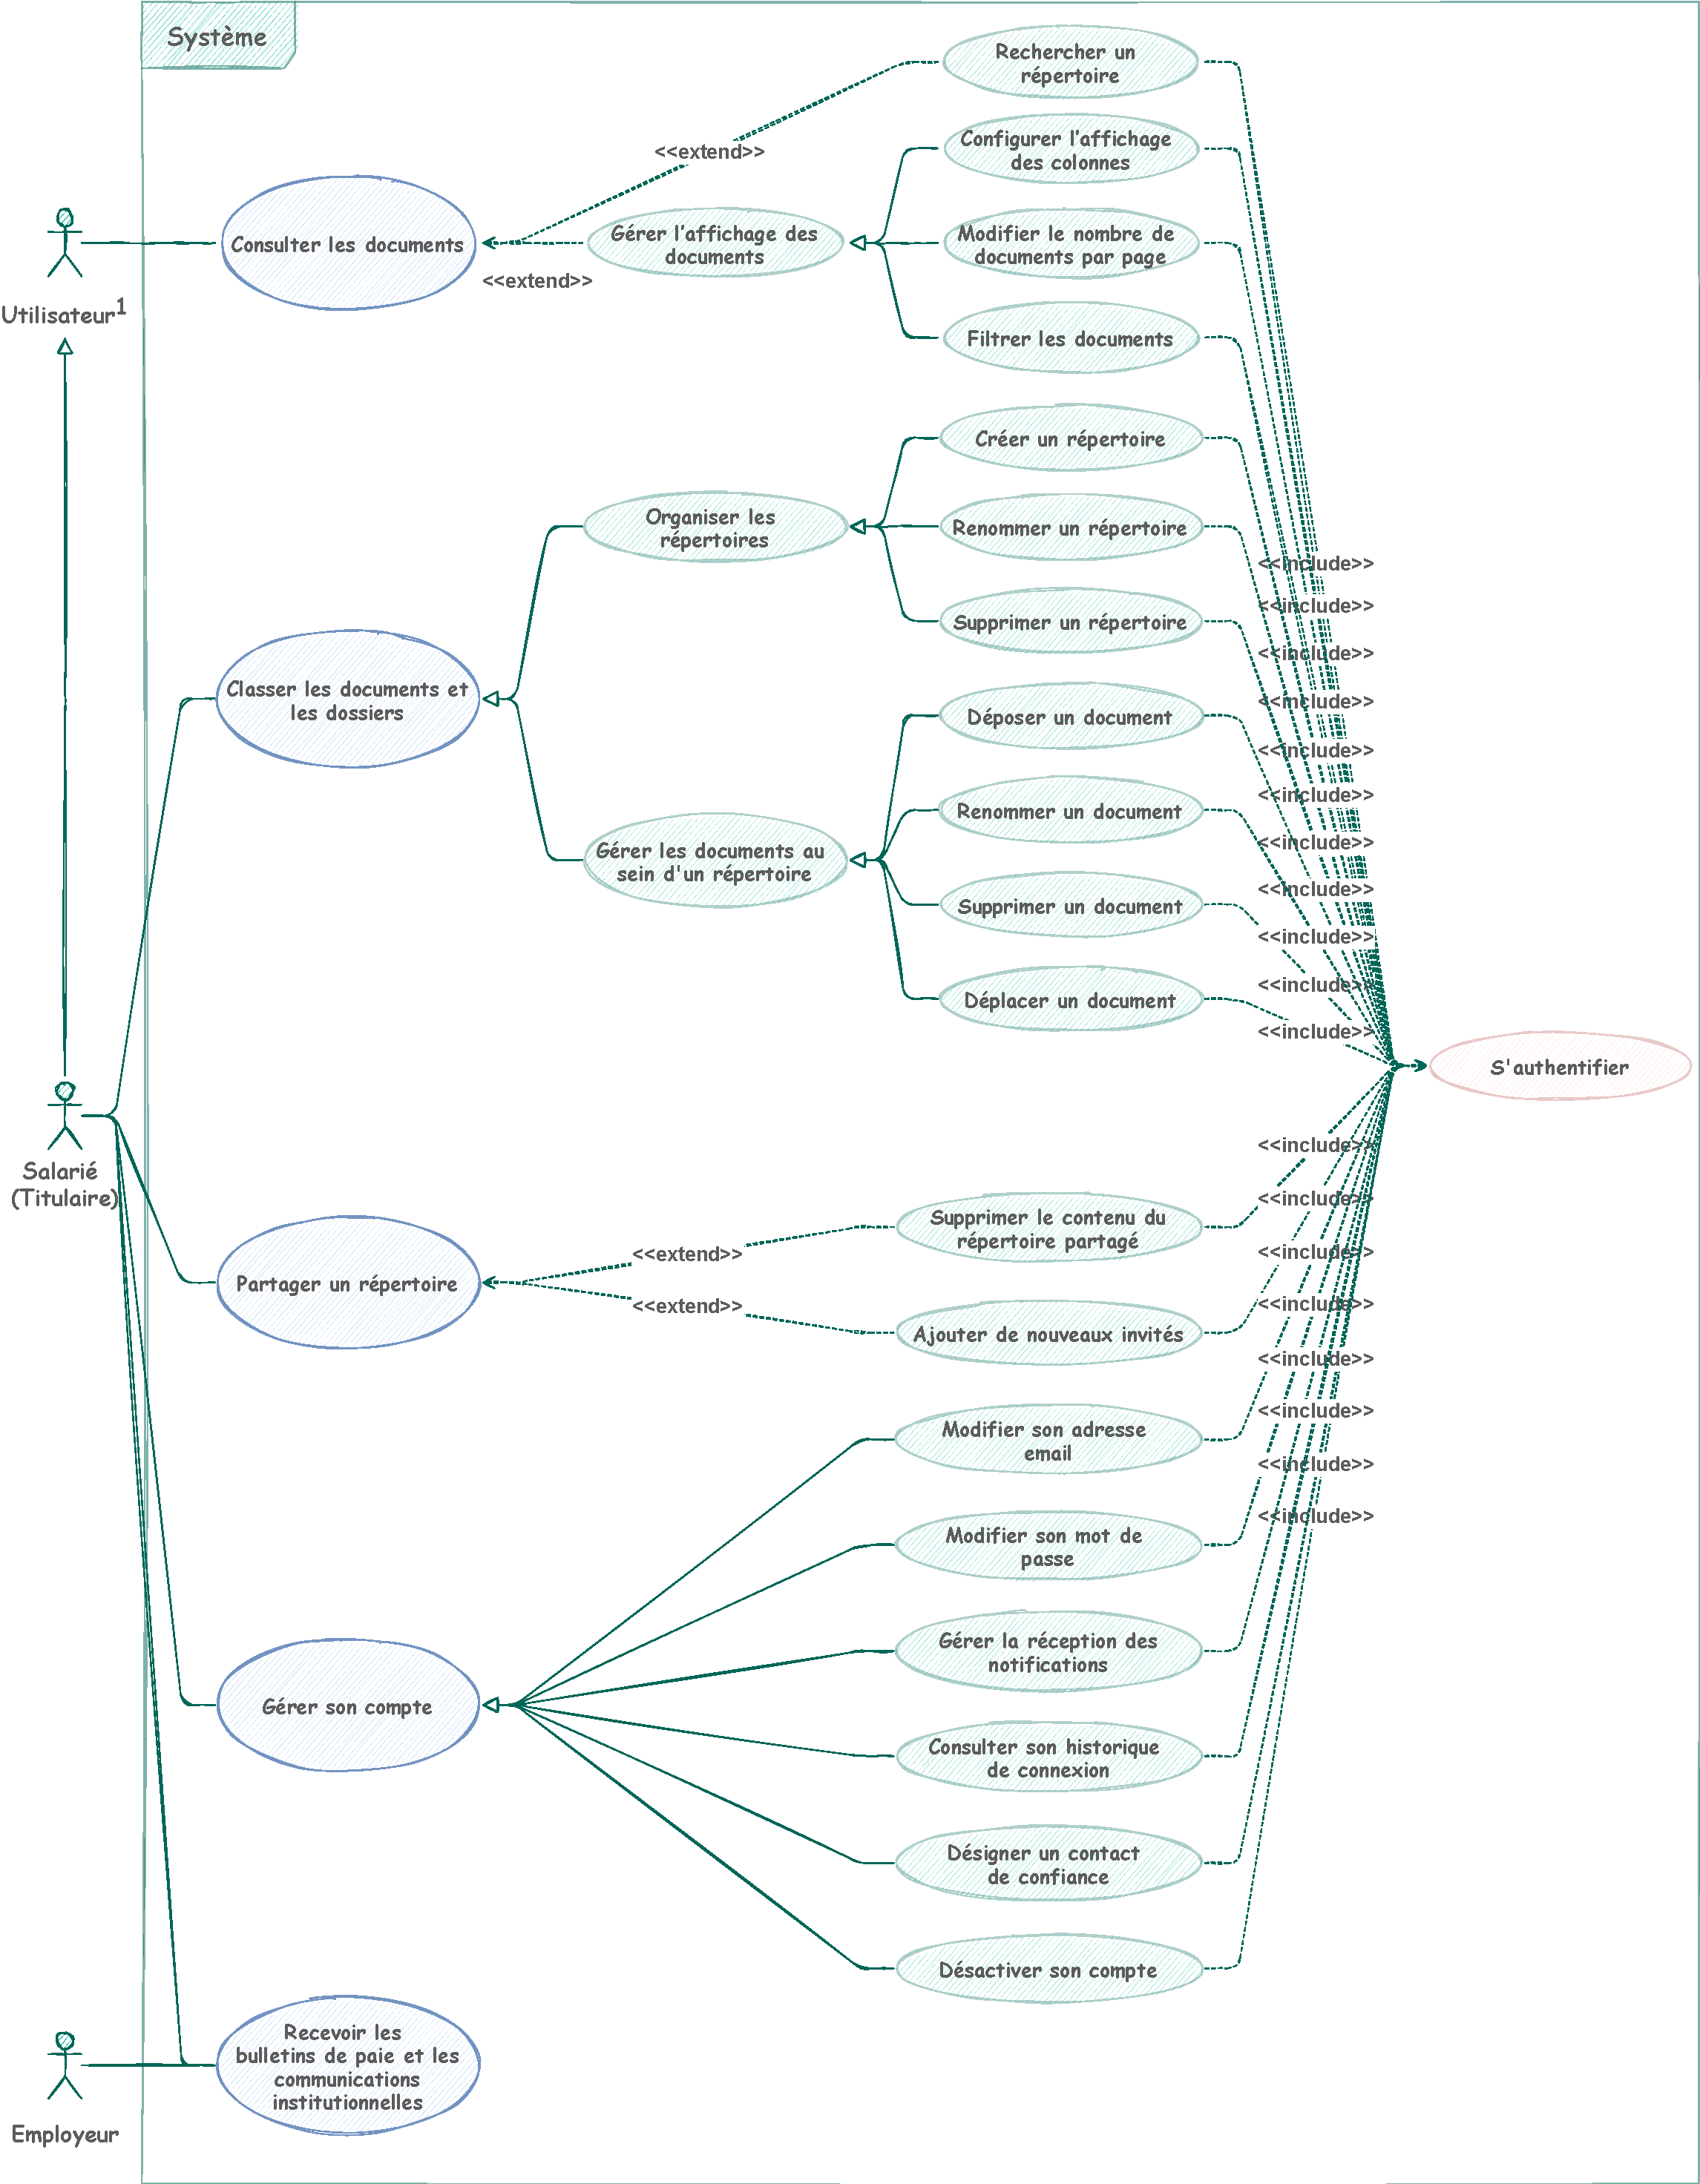
\includegraphics[width=1.1\linewidth]{images/sec3/usecase.pdf}
    \caption{Diagramme de cas d'utilisation général}
\end{figure}
\footnotetext[1]{représente le cas d'un acteur (non propriétaire) autorisé à utiliser le compte.}
\newpage
\subsubsection{Raffinement des cas d'utilisation prioritaires}
\definecolor{arkevia-btn-border}{HTML}{a3d7de}
\definecolor{arkevia-btn-bg}{HTML}{1aa1b4}
\definecolor{arkevia-btn-bg2}{HTML}{453659}
\setlength{\fboxrule}{1pt}
\setlength{\fboxsep}{6pt}

\begin{longtblr}[caption={Description textuelle du cas d’utilisation « S'inscrire »},
    note{1} = {Le mot de passe doit comporter un minimum de 8 caractères et un maximum de 20 caractères, au moins une lettre, au moins un chiffre, au moins un caractère spécial parmi @\#\$\%\^\&+=?\_|!,;.:\/ et ne doit pas contenir d'espaces.}]{
    hlines = {0.5pt,chambray},
    vlines = {0.5pt,chambray},
    row{odd} = {bg=azure9},
    colsep=4pt,
    rowsep=4pt,
    colspec={Q[l]X[l]},
    rowspec={Q[m] Q[m] Q[m] Q[m] Q[m] Q[m]},
}
\textbf{Acteur} & Salarié (Titulaire) \\
\textbf{Objectif}& 
L'inscription permet aux salariés d'activer la mise à disposition de leurs bulletins de paie électroniques dans leurs coffres-forts.\\
\textbf{Pré-condition} & 
Disposer d'une connexion Internet et d'un navigateur.\\
\textbf{Scénario} & 
\begin{minipage}{\linewidth}
\raggedright
\begin{enumerate}[leftmargin=*]
    \item Le salarié se rend sur \url{www.myarkevia.com} à l'aide d'un navigateur.
    \item Le salarié clique sur \fcolorbox{arkevia-btn-border}{arkevia-btn-bg}{\textcolor{white}{\scriptsize\textbf{JE M'INSCRIS}}}.
    \item Le salarié renseigne le matricule et le code secret qui lui ont été communiqués par le service RH, soit par des courriers spécifiques, soit par son dernier bulletin de salaire papier.
    \item Le salarié doit tenir compte de la \textbf{convention de mise à disposition du bulletin de paie électronique par l’employeur} et cocher la case \textcolor{gray}{\faCheckSquare\ J’ai lu et j’accepte les conditions de la convention} pour pouvoir passer à l’étape suivante.
    \item Le salarié renseigne les champs obligatoires concernant son profil.
   \item Le salarié doit tenir compte des \textbf{Conditions Générales d’Utilisation} et cocher la  case \textcolor{gray}{\faCheckSquare\ J’accepte les conditions générales d’utilisation d’ARKEVIA} pour pouvoir passer à l’étape suivante.
   \item Le salarié saisit son mot de passe conformément aux règles de sécurité\TblrNote{1}, puis le confirme.
   \item Enfin, le salarié clique sur \fcolorbox{arkevia-btn-border}{arkevia-btn-bg}{\textcolor{white}{\scriptsize\textbf{VALIDER MON INSCRIPTION}}} pour confirmer son inscription.
\end{enumerate}
\end{minipage}
\\
\textbf{Exception} & \begin{minipage}{\linewidth}
\raggedright
\begin{itemize}[leftmargin=*]
    \item Ouvert aux seuls salariés des entreprises ayant conclues un contrat de services avec CEGEDIM SRH (« Service ARKEVIA »)
    \item Le salarié saisit un matricule ou un code secret invalide.
    \item Le salarié saisit un mot de passe non conforme aux règles de sécurité définies par le système.
\end{itemize}
\end{minipage}
\\
\textbf{Post-condition} & Le système redirige automatiquement le salarié vers la page de connexion.\\
\end{longtblr}


\begin{longtblr}[caption={Description textuelle du cas d’utilisation « Se connecter »}]{
    hlines = {0.5pt,chambray},
    vlines = {0.5pt,chambray},
    row{odd} = {bg=azure9},
    colsep=4pt,
    rowsep=4pt,
    colspec={Q[l]X[l]},
    rowspec={Q[m] Q[m] Q[m] Q[m] Q[m] Q[m]},
}
\textbf{Acteur} & Salarié, actuel ou passé, ayant ouvert et utilisant le coffre-fort électronique, et le cas échéant, les personnes physiques spécifiquement habilitées par le titulaire. \\
\textbf{Pré-condition} & 
\begin{minipage}{\linewidth}
\raggedright
\begin{itemize}[leftmargin=*]
    \item Avoir préalablement suivi la procédure d'inscription.
    \item Disposer d'une connexion Internet et d'un navigateur.
\end{itemize}
\end{minipage}
\\
\textbf{Scénario} & 
\begin{minipage}{\linewidth}
\raggedright
\begin{enumerate}[leftmargin=*]
    \item L'utilisateur se rend sur \url{www.myarkevia.com} à l'aide d'un navigateur.
    \item L'utilisateur saisit son adresse e-mail et son mot de passe.
    \begin{itemize}
        \item Si nécessaire, il peut cliquer sur l’oeil \faEye{ } dans le champ \textbf{Mot de passe} pour voir son mot de passe en toutes lettres et ainsi éviter des erreurs de saisie.
    \end{itemize}
   \item Le salarié clique sur \fcolorbox{arkevia-btn-border}{arkevia-btn-bg}{\textcolor{white}{\scriptsize\textbf{JE ME CONNECTE}}} pour confirmer son inscription.
\end{enumerate}
\end{minipage}
\\
\textbf{Exception} & \begin{minipage}{\linewidth}
\raggedright
\begin{itemize}[leftmargin=*]
    \item Le salarié entre un mot de passe ou un e-mail incorrect.
    \item Au-delà de trois tentatives erronées, le système suspecte un abus ou une utilisation illégale de la part de l'utilisateur et bloque donc l'accès au compte pour une période de 15 minutes.
\end{itemize}
\end{minipage}
\\
\textbf{Post-condition} & Le système redirige l'utilisateur vers la page d'acceuil de son compte.\\
\end{longtblr}


\begin{longtblr}[caption={Description textuelle du cas d’utilisation « Créer un nouveau répertoire »}, note{2} = {Les noms de répertoire ne peuvent pas contenir d'espaces, ni de caractères non conformes aux règles de nommage des fichiers Unix.}]{
    hlines = {0.5pt,chambray},
    vlines = {0.5pt,chambray},
    row{odd} = {bg=azure9},
    colsep=4pt,
    rowsep=4pt,
    colspec={Q[l]X[l]},
    rowspec={Q[m] Q[m] Q[m] Q[m] Q[m] Q[m]},
}
\textbf{Acteur} & Salarié (Titulaire) \\
\textbf{Objectif}& 
Permettre au salarié de créer ses propres répertoires afin de stocker et classer ses documents (bulletins de paie ou documents personnels qu'il a déposés dans son coffre-fort).\\
\textbf{Pré-condition} & 
S'authentifier avec un identifiant correct.\\
\textbf{Scénario} & 
\begin{minipage}{\linewidth}
\raggedright
\begin{enumerate}[leftmargin=*]
    \item Dans la section répertoire de l'écran, le salarié sélectionne le dossier sous lequel il souhaite créer un répertoire. Le dossier sélectionné est alors marqué en vert.
    \item Le salarié clique sur l’icône \faPlusSquareO { }\textbf{Créer un nouveau répertoire}.
    \item Le salarié renseigne le nom du nouveau répertoire.
   \item Le salarié clique sur \fcolorbox{arkevia-btn-bg}{arkevia-btn-bg}{\textcolor{white}{\scriptsize\textbf{Créer}}}.
\end{enumerate}
\end{minipage}
\\
\textbf{Exception} & \begin{minipage}{\linewidth}
\raggedright
\begin{itemize}[leftmargin=*]
    \item Le nom du répertoire est invalide\TblrNote{2}.
    \item Création d'un répertoire avec un nom qui existe déjà.
\end{itemize}
\end{minipage}
\\
\textbf{Post-condition} & Le système renvoie un message indiquant à l'utilisateur qu'il peut désormais déposer des fichiers dans son nouveau répertoire.\\
\end{longtblr}



\begin{longtblr}[caption={Description textuelle du cas d’utilisation « Déposer un document »}]{
    hlines = {0.5pt,chambray},
    vlines = {0.5pt,chambray},
    row{odd} = {bg=azure9},
    colsep=4pt,
    rowsep=4pt,
    colspec={Q[l]X[l]},
    rowspec={Q[m] Q[m] Q[m] Q[m] Q[m] Q[m]},
}
\textbf{Acteur} & Salarié (Titulaire) \\
\textbf{Objectif}& 
Permettre aux salariés d'importer leurs documents importants.\\
\textbf{Pré-condition} & 
S'authentifier avec un identifiant correct.\\
\textbf{Scénario} & 
\begin{minipage}{\linewidth}
\raggedright
\begin{enumerate}[leftmargin=*]
    \item Le salarié sélectionne un dossier sous lequel il souhaite importer ses documents.
    \item Le salarié clique sur \fcolorbox{white}{arkevia-btn-bg2}{\textcolor{white}{ \scriptsize\textbf{\faFileO { } Déposer un document}}}.
   \item Dans la fenêtre \textbf{Ajout d’un document}, le salarié clique sur \fcolorbox{gray6}{gray!20!white}{\scriptsize\textbf{Choisir un fichier}}.
   \item Le salarié parcourt ses répertoires et sélectionne un fichier. Il peut éventuellement sélectionner plusieurs fichiers en appuyant sur la touche Ctrl et en cliquant simultanément avec la souris sur les fichiers souhaités.
    \item Le salarié clique sur \fcolorbox{arkevia-btn-bg}{arkevia-btn-bg}{\textcolor{white}{\scriptsize\textbf{Ajouter}}}.
\end{enumerate}
\end{minipage}
\\
\textbf{Exception} & 
Le fichier dépasse la taille limite autorisée de 50 Mo.\\
\textbf{Post-condition} & Le système renvoie un message indiquant à l'utilisateur que les documents sont en cours d'importation, puis un autre message indiquant le statut de l'opération lorsqu'elle est terminée.
\end{longtblr}


\begin{longtblr}[caption={Description textuelle du cas d’utilisation « Gérer un document »}]{
    hlines = {0.5pt,chambray},
    vlines = {0.5pt,chambray},
    row{odd} = {bg=azure9},
    colsep=4pt,
    rowsep=4pt,
    colspec={Q[l]X[l]},
    rowspec={Q[m] Q[m] Q[m] Q[m] Q[m] Q[m]},
}
\textbf{Acteur} & Salarié (Titulaire) \\
\textbf{Objectif}& 
Permettre aux salariés d'importer leurs documents importants.\\
\textbf{Pré-condition} & 
S'authentifier avec un identifiant correct.\\
\textbf{Scénario} & 
\begin{minipage}{\linewidth}
\raggedright
\begin{enumerate}[leftmargin=*]
    \item Le salarié sélectionne un répertoire pour accéder à son contenu.
    \item Dans la partie \textbf{Détail du répertoire} de l’écran, Il peut cliquer sur :
    \begin{itemize}
        \item L’icône \textcolor{gray7}{\textbf{Consulter} \faEye{ }} pour consulter le document.
        \item L’icône \textcolor{gray7}{\textbf{Renommer} \faPencil{ }} pour renommer le document.
        \item L’icône \textcolor{gray7}{\textbf{Supprimer} \faTrash{ }} pour supprimer le document.
        \item Le \textbf{nom du document} et, tout en maintenant le clic, il peut le glisser-déposer dans un répertoire de son choix.
    \end{itemize}
\end{enumerate}
\end{minipage}
\\
\textbf{Exception} & 
\begin{minipage}{\linewidth}
\raggedright
\begin{itemize}[leftmargin=*]
    \item Les documents professionnels déposés par l'employeur ne peuvent pas être supprimés par le salarié.
    \item Le nom du document ne peut pas être renommé avec un nom qui existe déjà dans le répertoire parent.
\end{itemize}
\end{minipage}
\\
\textbf{Post-condition} & 
Pour chaque action effectuée, le système renvoie un message indiquant à l'utilisateur l'état de l'opération lorsqu'elle est terminée.//
\end{longtblr}


\begin{longtblr}[caption={Description textuelle du cas d’utilisation « Gérer l'affichage des documents »}, , note{3} = {Les filtres actifs s’affichent au-dessus de la section \textbf{Détail du répertoire}.}]{
    hlines = {0.5pt,chambray},
    vlines = {0.5pt,chambray},
    row{odd} = {bg=azure9},
    colsep=4pt,
    rowsep=4pt,
    colspec={Q[l]X[l]},
    rowspec={Q[m] Q[m] Q[m] Q[m] Q[m] Q[m]},
}
\textbf{Acteur} & Salarié (Titulaire) \\
\textbf{Objectif}& 
Permettre aux salariés de configurer l’affichage des colonnes du tableau \textbf{Détail du répertoire}, de filtrer les  documents ainsi que d'ajuster le nombre de documents affichés par page.
\\
\textbf{Pré-condition} & 
S'authentifier avec un identifiant correct.\\
\textbf{Scénario} & 
\begin{minipage}{\linewidth}
\raggedright
\begin{itemize}[leftmargin=*]
    \item Pour configurer l’affichage des colonnes : 
    \begin{enumerate}
        \item Le salarié sélectionne un répertoire pour en afficher le contenu dans le tableau \textbf{Détail du répertoire}.
        \item Le salarié clique sur la liste déroulante \textbf{Gérer les colonnes} et coche les colonnes qu'il souhaite afficher et décoche celles qu'il souhaite masquer.
    \end{enumerate}
    \item Si le répertoire contient un grand nombre de documents, ils sont alors affichés sur plusieurs pages que le salarié peut parcourir à l'aide des boutons situés sous le tableau. Pour plus de commodité, le salarié a la possibilité d'afficher plus de lignes dans le tableau et ainsi de réduire le nombre de pages. Pour ce faire :
    \begin{enumerate}
        \item Le salarié clique sur la liste déroulante \textbf{[X] lignes}.
        \item Le salarié sélectionne 5, 10 ou 20 lignes.
    \end{enumerate}
    \item Le salarié a également la possibilité de filtrer les documents pour n'afficher que ceux correspondant aux critères de sélection qu'il a choisis. Pour ce faire :
    \begin{enumerate}
        \item Le salarié clique sur le bouton \fcolorbox{arkevia-btn-bg}{arkevia-btn-bg}{\textcolor{white}{\scriptsize\textbf{Filtrer } \faSliders}}.
        \item Parmi les 5 filtres proposés, le salarié clique sur les filtres souhaités. 
        \item Dans le champ qui s’affiche, le salarié renseigne les critères de filtrage.
        \item Le salarié clique  sur \fcolorbox{arkevia-btn-bg}{arkevia-btn-bg}{\textcolor{white}{\scriptsize\textbf{Appliquer les filtres}}}\TblrNote{3}.
        \item Le salarié clique sur la croix \textcolor{gray}{\faClose} pour fermer le volet des filtres.
    \end{enumerate}
    \item Pour désactiver le filtrage :
    \begin{enumerate}
        \item Le salarié clique sur le bouton \fcolorbox{arkevia-btn-bg}{arkevia-btn-bg}{\textcolor{white}{\scriptsize\textbf{Filtrer } \faSliders}} pour afficher le volet des filtres.
        \item Pour désactiver tous les filtres, le salarié clique sur le bouton Annuler \fcolorbox{arkevia-btn-bg}{white}{\textcolor{gray}{\faRefresh}}.
        \item Le salarié peut également désactiver certains filtres en cliquant sur le filtre à désactiver puis sur la croix \fcolorbox{white}{arkevia-btn-bg}{\textcolor{white}{\faClose}} pour supprimer les critères saisis.
A la fin, l'employé clique sur Appliquer les filtres pour rafraîchir la liste des documents.
\item Le salarié clique sur la croix \textcolor{gray}{\faClose} pour fermer le volet des filtres.
    \end{enumerate}
\end{itemize}
\end{minipage}
\\
\textbf{Exception} & Aucune
\\
\textbf{Post-condition} & 
Pour chaque action effectuée, l’affichage est instantanément modifié.
\end{longtblr}

\begin{longtblr}[caption={Description textuelle du cas d’utilisation « Partager un répertoire »},
note{4} = {La date saisie doit être postérieure à la date du jour.},
note{5} = {En ajoutant des documents au dossier  partagé, l'utilisateur crée simplement une copie des documents d'origine. Ils ne sont en aucun cas supprimés du répertoire d’origine.},
note{6} = {Il est impératif de cocher la case Envoyer une notification aux invités, sinon ils ne recevront pas de notification pour télécharger les documents qui leur sont partagés.}]{
    hlines = {0.5pt,chambray},
    vlines = {0.5pt,chambray},
    row{odd} = {bg=azure9},
    colsep=4pt,
    rowsep=4pt,
    colspec={Q[l]X[l]},
    rowspec={Q[m] Q[m] Q[m] Q[m] Q[m] Q[m]},
}
\textbf{Acteur} & Salarié (Titulaire) \\
\textbf{Objectif}& 
Donnez aux salariés la possibilité de créer des répertoires de partage afin qu'ils puissent partager des documents avec des tiers en dehors de leur entreprise.\\
\textbf{Pré-condition} & 
S'authentifier avec un identifiant correct.\\
\textbf{Scénario} & 
\begin{minipage}{\linewidth}
\raggedright
\begin{enumerate}[leftmargin=*]
    \item Le salarié doit d'abord créer un répertoire partagé, cela peut être fait à travers le scénario suivant :
    \begin{enumerate}
        \item Dans la liste des répertoires, le salarié clique sur le dossier \textbf{Partage}.
        \item Le salarié clique sur l’icône \textbf{Ajouter un répertoire partagé} \faShareAltSquare.
        \item Dans la fenêtre \textbf{Nouveau partage}, le salarié renseigne les champs suivants :
        \begin{itemize}
            \item \textbf{Nom du répertoire}.
            \item \textbf{Liste des invités} : il saisit les adresses e-mail des personnes avec lesquelles il souhaite partager ses documents, séparées par une virgule.
            \item \textbf{Commentaire}.
            \item \textbf{Date d’expiration du partage} : il saisit la date\TblrNote{4} jusqu’à laquelle le tiers pourra accéder au contenu de son répertoire de partage.
        \end{itemize}
        \item Le salarié clique sur \fcolorbox{arkevia-btn-bg}{arkevia-btn-bg}{\textcolor{white}{\scriptsize\textbf{Créer}}}.
    \end{enumerate}
    \item Pour ajouter des documents dans le répertoire partagé, le salarié sélectionne et glisse les documents vers le répertoire partagé précédemment créé\TblrNote{5}.
    \item Le salarié clique sur l’icône \textbf{Invitation partage} {\hspace{2pt}}\faFileTextO {\hspace{-13pt}\footnotesize\faInfoCircle}{\hspace{6pt}.}
    \item Éventuellement, le salarié peut :
    \begin{itemize}
        \item Ajouter de nouveaux e-mails d'invités dans le champ \textbf{Liste d’invités}.
        \item Modifiez la date d’expiration du partage.
    \end{itemize}
    \item Le salarié coche la case \textbf{Envoyer une notification aux invités}\TblrNote{6}.
    \item Le salarié clique sur \fcolorbox{arkevia-btn-bg}{arkevia-btn-bg}{\textcolor{white}{\scriptsize\textbf{Mettre à jour}}}.
\end{enumerate}
\end{minipage}
\\
\textbf{Exception} & 
    L'utilisateur inscrit un e-mail dont le format est considéré comme invalide.\\
\textbf{Post-condition} & 
Les invités reçoivent un mail contenant un lien de téléchargement des documents partagés qui sera actif jusqu’à la date d’expiration du partage. Une fois la date d’expiration atteinte, le répertoire partagé est supprimé du dossier \textbf{Partage}.
\end{longtblr}


\begin{longtblr}[caption={Description textuelle du cas d’utilisation « Supprimer un partage »}, note{7} = {Pour supprimer tous les documents du dossier partagé, le salarié doit supprimer individuellement chaque document contenu au sein du répertoire.}]{
    hlines = {0.5pt,chambray},
    vlines = {0.5pt,chambray},
    row{odd} = {bg=azure9},
    colsep=4pt,
    rowsep=4pt,
    colspec={Q[l]X[l]},
    rowspec={Q[m] Q[m] Q[m] Q[m] Q[m] Q[m]},
}
\textbf{Acteur} & Salarié (Titulaire) \\
\textbf{Objectif}& 
Supprimer tout ou partie des documents partagés avec un tiers avant la date d'expiration du partage.\\
\textbf{Pré-condition} & 
S'authentifier avec un identifiant correct.\\
\textbf{Scénario} & 
\begin{minipage}{\linewidth}
\raggedright
\begin{enumerate}[leftmargin=*]
    \item Le salarié sélectionne le dossier partagé dans le dossier \textbf{Partage}.
    \item Dans la section \textbf{Détail du répertoire}, le salarié clique sur l’icône \textcolor{gray7}{\textbf{Supprimer} \faTrash{ }} pour supprimer le document du répertoire\TblrNote{7}.
\end{enumerate}
\end{minipage}
\\
\textbf{Exception} & Aucune.\\
\textbf{Post-condition} & 
Le répertoire partagé restera visible dans la liste des répertoires partagés jusqu'à ce que la date d'expiration du partage soit atteinte. Si les invités cliquent sur le lien de téléchargement, le répertoire téléchargé ne contiendra pas les documents supprimés ou sera vide si le salarié a choisi de supprimer tous les documents.
\end{longtblr}
\subsubsection{Modélisation des processus métier}
\subsubsubsection{Diagramme de séquences modélisant le processus d'authentification}
\subsubsubsection{Diagramme de séquences modélisant ...}
\subsubsection{Diagramme de classe}
\subsection{Analyse des besoins}
\subsubsection{Migration du socle technique}
En voici les principaux changements sont les suivants :
cette migration sera donc accompagnée par d'autres migrations surtout les dépendances liées au framework Spring.​
\subsubsection{Factorisation et nettoyage du code}
\subsubsection{Optimisation du mécanisme d'envoi des notifications}
Le traitement par lot, communément appelé Batch dans le jargon informatique, est une problématique très répandue et quasiment incontournable au sein des entreprises et industries qui manipulent d'énormes masses de données. Dans cette section, nous allons vous présenter au travers d'un exemple d'application, la technologie Spring Batch/Spring Boot permettant de répondre à ce type de besoin. Cet article ne se veut pas et ne peut pas être exhaustif, car il s'agit d'une technologie immensément vaste. Mais les différents concepts présentés dans ce cours sont suffisants pour son appropriation.
\subsection{Conclusion}
%%%%%%%%%%%%%%%%%%
